\begin{wrapfigure}{r}{0.6\textwidth}
  % Requires \usepackage{graphicx}
  \centering
  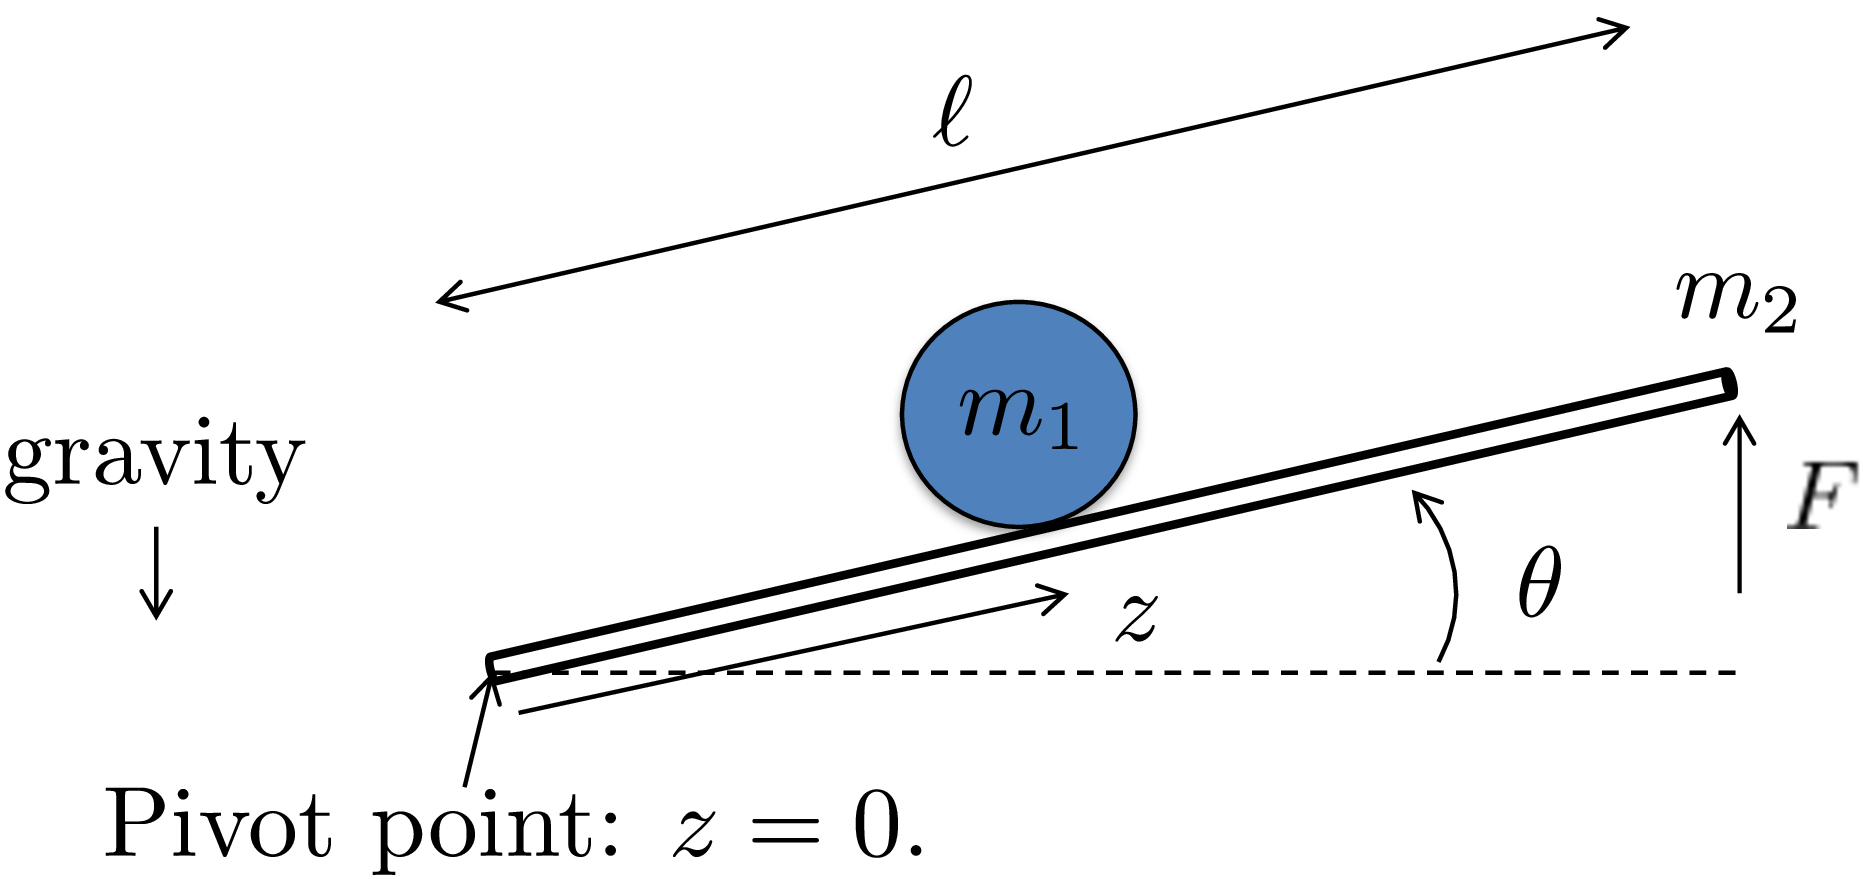
\includegraphics[width=0.59\textwidth]{6_design_studies/figures/hw_ballbeam_defn}\\
  \caption{Ball on Beam Problem}
  \label{fig:ballbeam_defn}
\end{wrapfigure}

%\controlbookfigure{0.5}
%	{6_design_studies/figures/hw_ballbeam_defn}
%	{Ball on Beam.}
%	{fig:ballbeam_defn}

Figure~\ref{fig:ballbeam_defn} shows the \index{ball and beam} system.  The position of the ball measured from the pivot point is $z$ and the speed of the ball along the direction of the beam is $\dot{z}$.  The angle of the beam from level is $\theta$ and the angular speed of the beam is $\dot{\theta}$.  Gravity acts in the down direction.  The mass of the ball is $m_1$ and the mass of the beam is $m_2$.  The length of the beam is $\ell$.  An external force is applied at the end of the beam as shown in \fref{fig:ballbeam_defn}.  

Use the following physical parameters: $m_1=0.35$~kg, $m_2=2$~kg, $\ell=0.5$~m, $g=9.8$~m/s$^2$.

